%!TEX program = xelatex
\documentclass{ctexart} % say 
\usepackage{tikz} 
\usepackage{xcolor}
\usetikzlibrary{decorations.text}
\usetikzlibrary{shapes}
\setmainfont{Athelas}

\begin{document}
\zihao{-2}
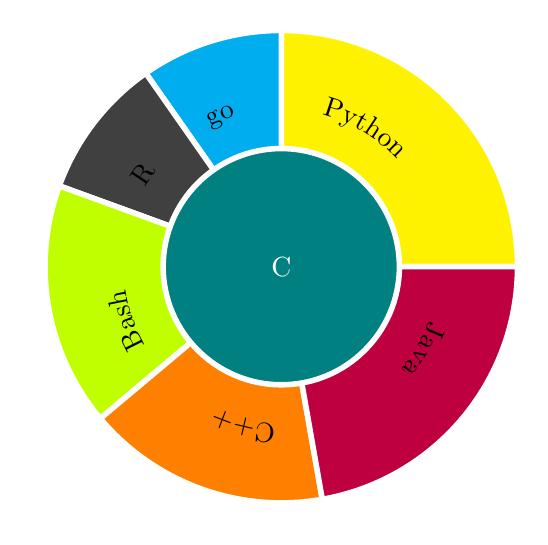
\begin{tikzpicture}

\fill [fill=yellow,draw=white,line width=2pt] (0,0) -- (0:3)  arc (0:90:3) -- (0,0);
\draw [decorate,decoration={text along path,
text={Python}}] (75:2) arc (75:0:2);
\fill[fill=cyan,draw=white,line width=2pt] (0,0) -- (90:3)  arc [start angle=90, end angle=125, radius=3] -- (0,0);
\draw [decorate,decoration={text along path,
text={go}}] (117:2) arc (117:0:2);
\fill[fill=darkgray,draw=white,line width=2pt] (0,0) -- (125:3)  arc [start angle=125, end angle=160, radius=3] -- (0,0);
\draw [decorate,decoration={text along path,
text={R}}] (150:2) arc (150:0:2);
\fill[fill=lime,draw=white,line width=2pt] (0,0) -- (160:3)  arc [start angle=160, end angle=220, radius=3] -- (0,0);

\draw [decorate,decoration={text along path,
text={Bash}}] (210:2) arc (210:0:2);

\fill[fill=orange,draw=white,line width=2pt] (0,0) -- (220:3)  arc [start angle=220, end angle=280, radius=3] -- (0,0);

\draw [decorate,decoration={text along path,
text={C++}}] (268:2) arc (268:0:2);
\fill[fill=purple,draw=white,line width=2pt] (0,0) -- (280:3)  arc [start angle=280, end angle=360, radius=3] -- (0,0);
\draw [decorate,decoration={text along path,
text={Java}}] (340:2) arc (340:0:2);
\filldraw[fill=teal,draw=white,line width=2pt] (0,0) circle [radius=3*0.5];
\zihao{0}
\draw (0,0) node[white] {C};

\end{tikzpicture}

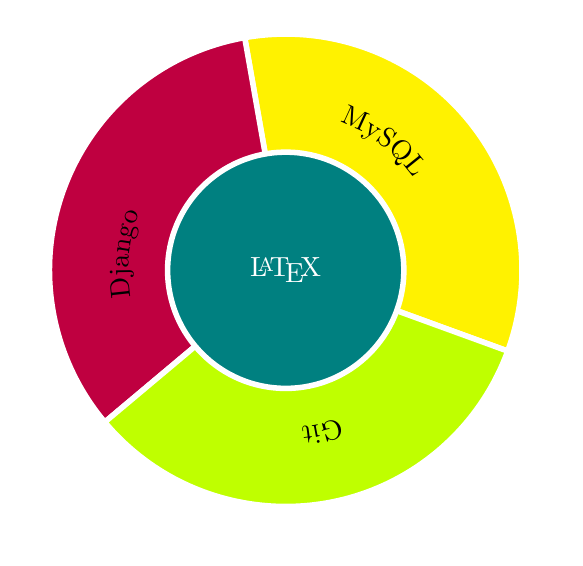
\begin{tikzpicture}

\fill [fill=yellow,draw=white,line width=2pt] (0,0) -- (-20:3)  arc (-20:100:3) -- (0,0);
\draw [decorate,decoration={text along path,
text={MySQL}}] (70:2) arc (70:0:2);
\fill[fill=purple,draw=white,line width=2pt] (0,0) -- (100:3)  arc [start angle=100, end angle=220, radius=3] -- (0,0);
\draw [decorate,decoration={text along path,
text={Django}}] (190:2) arc (190:0:2);
\fill[fill=lime,draw=white,line width=2pt] (0,0) -- (220:3)  arc [start angle=220, end angle=340, radius=3] -- (0,0);
\draw [decorate,decoration={text along path,
text={Git}}] (290:2) arc (290:0:2);
\filldraw[fill=teal,draw=white,line width=2pt] (0,0) circle [radius=3*0.5];
\zihao{1}
\draw (0,0) node[white] {\LaTeX};

\end{tikzpicture}



\begin{tikzpicture}
\node [star, star point height=.5cm, minimum size=2cm, fill,cyan]
       at (1,1) {};
\node [star, star point height=.5cm, minimum size=2cm, fill,cyan]
       at (3,1) {};
\node [star, star point height=.5cm, minimum size=2cm, fill,cyan]
       at (5,1) {};
\node [star, star point height=.5cm, minimum size=2cm, fill,cyan]
       at (7,1) {};
\node [star, star point height=.5cm, minimum size=2cm, fill,cyan]
       at (9,1) {};
\end{tikzpicture}



\begin{tikzpicture}
\node [star, star point height=.5cm, minimum size=2cm, fill,cyan]
       at (1,1) {};
\node [star, star point height=.5cm, minimum size=2cm, fill,cyan]
       at (3,1) {};
\node [star, star point height=.5cm, minimum size=2cm, fill,cyan]
       at (5,1) {};
\node [star, star point height=.5cm, minimum size=2cm, fill,cyan]
       at (7,1) {};
\node [star, star point height=.5cm, minimum size=2cm, fill,gray]
       at (9,1) {};
\end{tikzpicture}


\begin{tikzpicture}
\node [star, star point height=.5cm, minimum size=2cm, fill,cyan]
       at (1,1) {};
\node [star, star point height=.5cm, minimum size=2cm, fill,cyan]
       at (3,1) {};
\node [star, star point height=.5cm, minimum size=2cm, fill,cyan]
       at (5,1) {};
\node [star, star point height=.5cm, minimum size=2cm, fill,gray]
       at (7,1) {};
\node [star, star point height=.5cm, minimum size=2cm, fill,gray]
       at (9,1) {};
\end{tikzpicture}



\begin{tikzpicture}
\node [star, star point height=.5cm, minimum size=2cm, fill,cyan]
       at (1,1) {};
\node [star, star point height=.5cm, minimum size=2cm, fill,cyan]
       at (3,1) {};
\node [star, star point height=.5cm, minimum size=2cm, fill,gray]
       at (5,1) {};
\node [star, star point height=.5cm, minimum size=2cm, fill,gray]
       at (7,1) {};
\node [star, star point height=.5cm, minimum size=2cm, fill,gray]
       at (9,1) {};
\end{tikzpicture}



\begin{tikzpicture}
\node [star, star point height=.5cm, minimum size=2cm, fill,cyan]
       at (1,1) {};
\node [star, star point height=.5cm, minimum size=2cm, fill,gray]
       at (3,1) {};
\node [star, star point height=.5cm, minimum size=2cm, fill,gray]
       at (5,1) {};
\node [star, star point height=.5cm, minimum size=2cm, fill,gray]
       at (7,1) {};
\node [star, star point height=.5cm, minimum size=2cm, fill,gray]
       at (9,1) {};
\end{tikzpicture}
\end{document}